\graphicspath{{./ch_adptv_msmnt_cntrl/figures/}}


\chapter[Manipulating a qubit through the backaction of adaptive measurements]{Manipulating a qubit through the backaction of sequential partial measurements \\ and real-time feedback }
\label{ch:AMC}

\begin{center} 
    \vspace{-1cm} {M.S.~Blok$^*$, C.~Bonato$^*$, M.L.~Markham, D.J. ~Twitchen, V.V. ~Dobrovitski and R.~Hanson} 
\end{center}


{\renewcommand{\thefootnote}{}\footnote{This chapter has been published in
    {\em Nature Physics} \textbf{10}, 189-193 (2014).}\footnote{$^*$ these authors contributed equally to this work}}


\vspace{-0.5cm} 
Quantum measurements not only extract information from a system but also alter its state. Although the outcome of the measurement is probabilistic, the backaction imparted on the measured system is accurately described by quantum theory ~\cite{Guerlin_Nature_2007,Hatridge_Science_2013,Murch_Nature_2013}. Therefore, quantum measurements can be exploited for manipulating quantum systems without the need for control fields~\cite{Ashhab_PhysRevA_2010,Wiseman_NatureNV_2011}. We demonstrate measurement-only state manipulation on a nuclear spin qubit in diamond by adaptive partial measurements. We implement the partial measurement via tunable correlation with an electron ancilla qubit and subsequent ancilla readout~\cite{Brun_PhysRevA_2008,Groen_PRL_2013}. We vary the measurement strength to observe controlled wavefunction collapse and find post-selected quantum weak values~\cite{Brun_PhysRevA_2008,Groen_PRL_2013,Aharonov_PRL_1988,Pryde_PRL_2005,Dressel_ArXiv_2013}. By combining a novel quantum non-demolition readout on the ancilla with real-time adaption of the measurement strength we realize steering of the nuclear spin to a target state by measurements alone. Besides being of fundamental interest, adaptive measurements can improve metrology applications~\cite{Cappellaro_PhysRevA_2012,Higgins_Nature_2007} and are key to measurement-based quantum computing~\cite{Raussendorf_PRL_2001,Prevedel_Nature_2007}.


\clearpage

\section{Introduction}
Measurements play a unique role in quantum mechanics and in quantum information processing. The backaction of a measurement can be used for state initialization~\cite{Robledo_Nature_2011,Riste_PRL_2012}, generation of entanglement between non-interacting systems~\cite{Chou_Nature_2005,Moehring_Nature_2007,Pfaff_NatPhys_2012,Riste_Nature_2013}, and for qubit error detection~\cite{Chiaverini_Nature_2004}. These measurement-based applications require either post-selection or real-time feedback, as the outcome of a measurement is inherently probabilistic. Recent experiments achieved quantum feedback control on a single quantum system~\cite{Riste_Nature_2013, Gillett_PRL_2010,Sayrin_Nature_2011,Vijay_Nature_2012} by performing coherent control operations conditioned on a measurement outcome.

Here, we realize real-time adaptive measurements and exploit these in a proof-of-principle demonstration of measurement-only quantum feedback. Our protocol makes use of partial measurements that balance the information gain and the measurement backaction by varying the measurement strength. We accurately control the measurement strength and the corresponding backaction in a two-qubit system by tuning the amount of (quantum) correlation between the system qubit and an ancilla qubit, followed by projective readout of the ancilla~\cite{Brun_PhysRevA_2008,Groen_PRL_2013}. In general, the backaction of sequential partial measurements leads to a random walk~\cite{Guerlin_Nature_2007,Hatridge_Science_2013,Murch_Nature_2013} but by incorporating feedback, multiple measurements can direct the trajectory of a qubit towards a desired state~\cite{Ashhab_PhysRevA_2010,Wiseman_NatureNV_2011}. Real-time adaptive measurements are a key ingredient for quantum protocols such as one-way quantum computing~\cite{Raussendorf_PRL_2001,Prevedel_Nature_2007} and Heisenberg-limited phase estimation~\cite{Cappellaro_PhysRevA_2012,Higgins_Nature_2007}.

We implement the adaptive partial measurements in a nitrogen vacancy (NV) center in synthetic diamond. We define the system qubit by the nuclear spin of the NV host nitrogen ($\ket{\downarrow}$: $m_I$=0, $\ket{\uparrow}$: $m_I$= -1), and the ancilla qubit by the NV electron spin ($\ket{0}$: $m_S$=0, $\ket{1}$: $m_S$=-1) (Fig.\,\ref{fig:amc-fig1}a). The ancilla is initialized and read out in a single shot with high fidelity using spin-selective optical transitions~\cite{Robledo_Nature_2011}. We perform single-qubit operations on the ancilla by applying microwave frequency pulses to an on-chip stripline.


\section{Variable-strength measurement}
\begin{figure*}
	\centering
	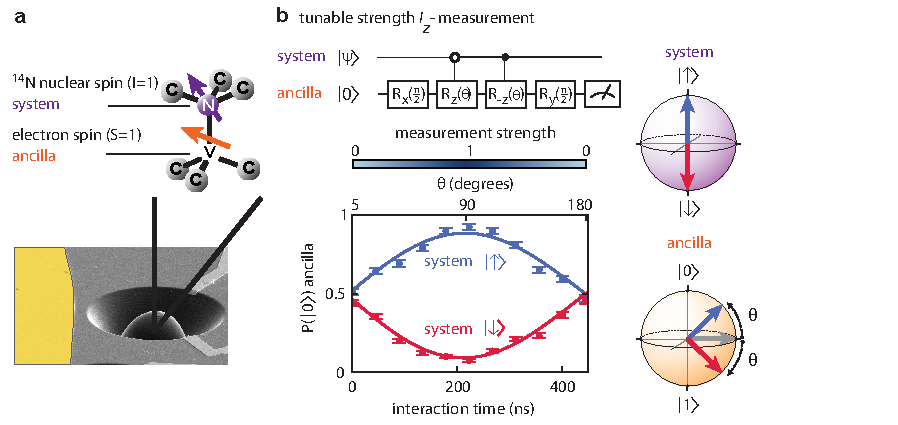
\includegraphics{fig1_twocolumns}
	\caption{\label{fig:amc-fig1} \textbf{Partial measurement of a spin qubit in diamond.} (a) The NV center is a natural two-qubit system where the system qubit is defined by the $^{14}N$ nuclear spin and the ancilla qubit is defined by the electron spin. A solid-immersion-lens is deterministically fabricated on top of the selected NV center to increase the photon collection efficiency. Control fields for single qubit rotations are generated by applying a current to the gold stripline (yellow).  (b) A tunable strength measurement is implemented by a Ramsey-type gate on the ancilla. We plot the probability to measure the state $\ket{0}$  for the ancilla, as a function of interaction time $\tau$, for two system input states $\ket{\downarrow}$ (red) and $\ket{\uparrow}$ (blue). The Bloch-spheres show the state of the system (purple) and ancilla (orange) after the entangling-gate for the different input states (red and blue vectors). The colour bar represents the measurement strength, proportional to $\sin{\theta}$, where $\theta=\frac{A \tau}{2}$. Blue corresponds to a projective measurement and white to no measurement. Solid lines are a  fit to the function $y_0 + e^{-( \frac{\tau}{T_2^*})^2} \cos{(A \tau + \delta)} $. From the phase offset $\delta$ we find the weakest measurement we can perform, corresponding to $\theta = 5^{\circ}$. This is limited by free evolution of the ancilla during the pulses.(see Methods). Error bars depict 68 $\%$ confidence intervals. Sample size is 500 for each data point. }
\end{figure*}

We realize the variable-strength measurement by correlating the system qubit with the ancilla through a controlled-phase-type gate (Fig.\,\ref{fig:amc-fig1}b) that exploits the hyperfine interaction, which (neglecting small off-diagonal terms) has the form $\hat{H}_{hf}=A\hat{S}_{z}\hat{I}_{z}$ (with $A = 2 \pi \times 2.184 \pm 0.002$ MHz and $\hat{S}_{z}, \hat{I}_{z}$ the three-level Pauli z-operators for the electron, nuclear spin respectively).  During free evolution, the ancilla qubit precession is conditional on the state of the system qubit. We choose the rotating frame such that the ancilla rotates clockwise (anti-clockwise) around the z-axis if the system qubit is in $\ket{\uparrow}$ ($\ket{\downarrow}$) and vary the interaction time $\tau$. For $\tau = 0$, there is no correlation between the ancilla and the system, whereas for $\tau = \frac{\pi}{A}$, corresponding to the rotation angle $\theta = 90^{\circ}$, the two are maximally correlated. A subsequent rotation and projective readout of the ancilla then implements a measurement of the system qubit, with a measurement strength that can be accurately tuned by controlling the interaction time $\tau$. A mathematical derivation  can be found in the methods.

We investigate the measurement-induced backaction by preparing an initial state of the system ($\ket{\up},\ket{x}$ and $\ket{y}$) and performing a partial measurement with strength $\theta$, followed by state tomography (Fig.\,\ref{fig:amc-fig2}a). First, we neglect the outcome of the partial measurement, which is mathematically equivalent to taking the trace over the state of the ancilla qubit. In this case the backaction is equivalent to pure dephasing as can be seen by a measured reduction of the length of the Bloch vector (Fig.\,\ref{fig:amc-fig2}b). Next, we condition the tomography on the ancilla measurement yielding state $\ket{0}$ (Fig.\,\ref{fig:amc-fig2}c). We observe that for a weak measurement $(\theta = 5^{\circ})$, the system is almost unaffected, whereas for increasing measurement strength it receives a stronger kick towards $\ket{\uparrow} $(Fig.\,\ref{fig:amc-fig2}c). Crucially, we find that the length of the Bloch vector is preserved in this process, as expected for an initially pure state. This shows that the partial collapse is equivalent to a qubit rotation that is conditional on the measurement strength and outcome and on the initial state. By performing quantum process tomography, we find that both measurement processes agree well with the theoretical prediction (the process fidelities are 0.986 $\pm$ 0.004 and 0.94 $\pm$ 0.01 for the unconditional and conditional process, respectively; see Methods).


\begin{figure}
	\centering
	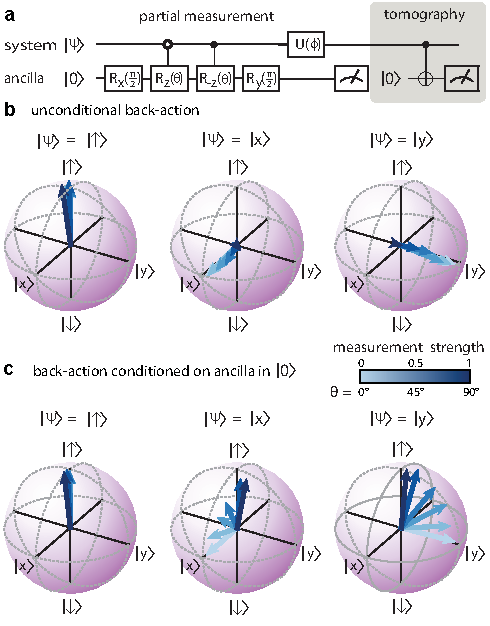
\includegraphics{fig2_partial_measurement_backaction}
	\caption{\label{fig:amc-fig2} \textbf{Measurement backaction for variable-strength measurement}. (a) We prepare an initial state  of the system ($\ket{\uparrow}$,  $\ket{x}$ and  $\ket{y}$), perform a partial measurement with strength $\theta$, and characterize the measurement backaction on the system by quantum state tomography. Quantum state tomography is implemented by an ancilla-assisted projective measurement, performed with the same protocol, setting $\tau = 229$ ns for $\theta = 90^{\circ}$. The nuclear spin basis rotation is performed with a $\frac{\pi}{2}$ radio-frequency pulse (along either $x$ or $y$). The basis rotation pulse for the tomography is applied before the readout of the ancilla, to avoid the dephasing induced by the state-characterization measurement (see main text). The data is corrected for errors in the readout and initialization of the system qubit, both of which are obtained from independent measurements (see methods). (b,c)  Measurement backaction for a partial measurement of increasing strength, independent of the measurement result for the ancilla qubit (b), or conditioned on the ancilla in  $\ket{0}$ (c). }
\end{figure}

\section{Generalized weak value}
By combining a partial measurement with post-selection on the outcome of a subsequent projective measurement, we can measure the generalized weak value $_{f} \langle I_{z} \rangle$ (conditioned average of contextual values \cite{Dressel_PRL_2010}, see methods) of the nuclear spin in the $z$-basis. In the limit of zero measurement strength ($\theta = 0^{\circ}$), this quantity approximates the weak value \cite{Aharonov_PRL_1988} $W = \frac{\bra{\psi_f} \hat{I}_z \ket{\psi_i}}{\bra{\psi_f} \psi_i \rangle}$ , where $ \psi_i (\psi_f )$ is the initial (final) state of the nucleus and from here we define $\hat{I}_z$ as the Pauli $z$-operator reduced to a two-level system with eigenvalues +1 and $-$1. By post-selecting only on the final states having small overlap with the initial state, $_{f} \langle I_{z} \rangle$ can be greatly amplified to values that lie outside the range of eigenvalues of the measured observable. As shown in Fig.\,\ref{fig:amc-fig3}, by sweeping the angle between the initial and final states we observe up to tenfold amplification ($_{f} \langle I_{z} \rangle = 10 \pm 3$) compared to the maximum eigenvalue of $I_{z}$ ($+1$). This amplification is the highest reported for a solid-state system to date\cite{Groen_PRL_2013}. As predicted \cite{Williams_PRL_2008}, we observe that values of  $_{f} \langle I_{z} \rangle$ lying outside of the range of eigenvalues of $I_{z}$ can be found for any finite measurement strength.

\begin{figure}
	\centering
	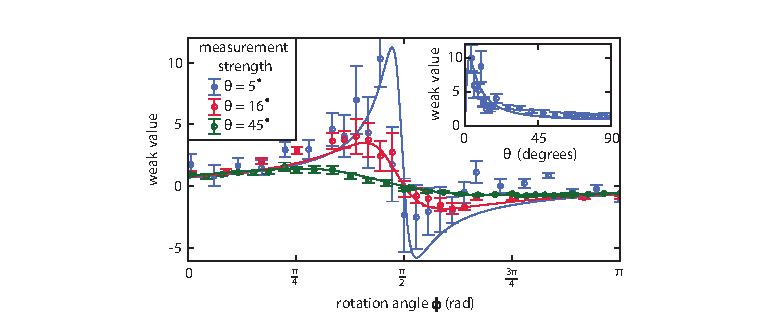
\includegraphics{fig3_weak_value}
	\caption{\label{fig:amc-fig3} \textbf{Generalized quantum weak value}. Measurement of a generalized weak value for the nuclear-spin qubit, performed by a partial measurement of strength $\theta$, followed by a strong measurement and post-selection of the state  $\ket{\downarrow}$, as a function of the basis rotation angle $\phi$ of the strong measurement (Fig.\,\ref{fig:amc-fig2}a). Solid lines are simulations using independently determined parameters. The asymmetry in the curve can be explained by asymmetric nuclear spin flips arising during ancilla initialisation by optical excitation of the forbidden transition of $E_{y}$ (see methods). Inset: the generalized weak values as a function of the strength $\theta$ of the partial measurement, setting the basis rotation angle of the strong measurement to the optimal value  $\phi = \frac{\pi}{2} - \theta$. All error bars depict 68 $\%$ confidence intervals. The sample size varies per data point because each data point has different post-selection criterion.}
\end{figure}

\section{QND-measurement of the ancilla qubit}
Using the partial measurements for measurement-based feedback requires reading out the ancilla without perturbing the system qubit. In our experiment the system qubit can dephase during ancilla readout both through a spin-flip of the electron in the course of optical excitation (Fig.\,\ref{fig:amc-fig4}b) and as a result of the difference in the effective nuclear g-factor in the electronic ground- and optically excited state~\cite{Jiang_PRL_2008}. Note that for the characterization of a single partial measurement (Fig.\,\ref{fig:amc-fig2}) we circumvent this dephasing by interchanging the measurement basis rotation and the ancilla readout; this interchange is not possible for real-time adaptive measurements.

\begin{figure*}
	\centering
	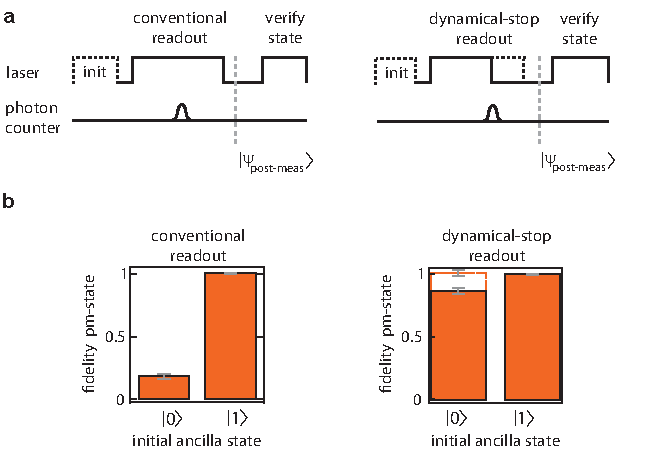
\includegraphics{fig4_qnd_electron}
	\caption{\label{fig:amc-fig4} \textbf{Quantum non-demolition measurement of the ancilla qubit} (a) The ancilla is initialized in $\ket{0}$ ($\ket{1}$) by optically pumping the $A_2$ ($E_y$) transition. The ancilla is then read out by exciting the $E_y$ transition for 100 $\mu$s (conventional readout), or until a photon was detected (dynamical-stop readout). Finally, we verify the post-measurement state with a conventional readout. (b) Fidelity of the post-measurement state of the ancilla for conventional readout (left graph) and dynamical-stop readout (right graph). Results are corrected for the infidelity in the final readout.  All error bars depict 68 $\%$ confidence intervals. Sample size per datapoint is 5000 }
\end{figure*}

To mitigate the nuclear dephasing during ancilla readout we reduce the ancilla spin-flip probability using a dynamical-stop readout technique. We partition the optical excitation time in short ($1~ \mu$s) intervals and we stop the excitation laser as soon as a photon is detected, or after a predetermined maximum readout time when no photon is detected (Fig.\,\ref{fig:amc-fig4}a). This reduces redundant excitations without compromising the readout fidelity. In Fig.\,\ref{fig:amc-fig4}b we show the correspondence between pre- and post-measurement states for the two eigenstates of the ancilla. For the state $\ket{0}$ the dynamical-stop readout increases the fidelity ($F = \bra{\psi_i}\rho_m \ket{\psi_i}$, where $\rho_m$ is the density matrix of the system after the ancilla readout) from 0.18 $\pm$ 0.02 to 0.86 $\pm$ 0.02. The latter fidelity is solely limited by the cases where the spin flipped before a photon was detected: we find $F = 1.00 \pm 0.02$ for the cases in which a photon was detected. As expected, the fidelity is high ($F = 0.996 \pm 0.006$) for input state $\ket{1}$ as this state is unaffected by the excitation laser. The dynamical-stop technique thus implements a quantum non-demolition (QND) measurement of the ancilla electron spin with an average fidelity of 0.93 $\pm$ 0.01 for the post-measurement state.

The dynamical-stop readout of the ancilla significantly reduces the dephasing of the nuclear spin qubit during measurement as shown in Fig.\,\ref{fig:amc-fig5}. Starting with the nuclear spin in state $\ket{x} = \frac{\ket{0} + \ket{1}}{\sqrt{2}}$, a conventional readout of the ancilla completely dephases the nuclear spin, leading to a state fidelity with respect to $\ket{x}$ of 0.5. In contrast, the fidelity of the dynamical-stop readout saturates to 0.615 $\pm$ 0.002 (probably limited by changes in the effective g-factor of the nuclear spin). The dynamical-stop readout thus leaves the system in a coherent post-measurement state that can be used in a real-time feedback protocol. 

\begin{figure*}
	\centering
	\includegraphics{fig5_qnd_nuclear_spin}
	\caption{\label{fig:amc-fig5} \textbf{System qubit coherence during ancilla readout}. Coherence of the system qubit state after ancilla readout. For the dynamical-stop protocol we define the ancilla readout time as the predetermined maximum readout time. The graph shows the fidelity of the system with respect to $\ket{x}$ for conventional readout (red) and dynamical-stop readout (blue). The $z$-component of the system is unaffected as shown by the constant fidelity with respect to $\ket{\uparrow}$ (grey). All error bars depict 68 $\%$ confidence intervals. Sample size per datapoint is 2000 }
\end{figure*}

\section{Control by adaptive measurements}
Preserving coherence of the post-measurement state enables a proof-of-principle realization of measurement-only control, by implementing sequential measurements and tuning the strength of the second measurement in real time conditioned on the outcome of the first measurement (Fig.\,\ref{fig:amc-fig6}a). We choose as our target the creation of the state $\ket{\psi} = \cos{(\frac{\pi}{4}+\frac{\theta_1}{2})}\ket{\downarrow}+\cos{(\frac{\pi}{4}-\frac{\theta_1}{2})}\ket{\uparrow}$ from initial state $\ket{x}$ using only partial measurements of $\hat{I}_z$. The first measurement with strength $\theta_1$ will prepare either the desired state, or the state $\ket{\psi_{wrong}} =  \cos{(\frac{\pi}{4}-\frac{\theta_1}{2})}\ket{\downarrow}+\cos{(\frac{\pi}{4}+\frac{\theta_1}{2})}\ket{\uparrow}$ , each with probability 0.5. We adapt the strength of the second measurement $\theta_2$ according to the outcome of the first measurement: we set $\theta_2 = 0$ if the first measurement directly yielded the target state, but if the wrong outcome was obtained we set the measurement strength to

\begin{equation}
\theta_2 = \sin{^{-1}\left[2 \frac{\sin{\theta_1}}{1 + \sin{^2 \theta_1}}\right]},
\end{equation}

such that the second measurement will probabilistically rotate the qubit to the target state (see methods). The total success probability of this two-step protocol is  $p_{suc} = \frac{1}{2}(1 + \cos{\theta_1})$ and a successful event is heralded by the outcome of the ancilla readout. In principle the protocol can be made fully deterministic~\cite{Ashhab_PhysRevA_2010} by incorporating a reset in the form of a projective measurement along the $x$-axis.

To find the improvement achieved by the feedback, we first compare the success probability of our adaptive measurement protocol to the success probability for a single measurement (Fig.\,\ref{fig:amc-fig6}b right panel). The success probability clearly increases with the adaptive protocol and is proportional to the readout fidelity of the $\ket{0}$ state of the ancilla, which is maximum for readout times  \textgreater~25~$\mu$s. The fidelity of the final state (Fig.\,\ref{fig:amc-fig6}b left panel) is limited by the remaining dephasing of the system during readout of the ancilla as shown in Fig.\,\ref{fig:amc-fig5}. This constitutes the trade-off between success probability and state fidelity. 

We show that the increase in success probability is enabled by feedback by comparing the final state fidelity with and without feedback (Fig.\,\ref{fig:amc-fig6}b left panel). In principle the success probability can be increased in the absence of feedback by accepting a certain number of false measurement outcomes at the cost of a reduced fidelity. We calculate the maximum fidelity that can be achieved in this way by performing only the first measurement and increasing the success probability to that of the adaptive protocol using post-selection (grey line in Fig.\,\ref{fig:amc-fig6}b, left panel). We find that the measured state fidelity in the adaptive protocol is above this bound (Fig.\,\ref{fig:amc-fig6}b, green area), which indicates that the adaptive measurement indeed successfully corrects the kickback from the first measurement, thus yielding a clear advantage over open-loop protocols.



We note that, in contrast to pioneering adaptive measurement experiments on photons that only used experimental runs in which a photon was detected at each measurement stage~\cite{Prevedel_Nature_2007}, our protocol is fully deterministic in the sense that the partial measurement always yields an answer. In particular, the data in Fig.\,\ref{fig:amc-fig6} includes all experimental runs and thus no post-selection is performed, as desired for future applications in metrology and quantum computing. 

The performance of the protocol can be further improved by increasing the ancilla readout fidelity (either by improving the collection efficiency or reducing spin-flip probability) and by further reducing the dephasing of the system during readout. A particularly promising route is to use nuclear spins farther away from the NV center (for example carbon-13 spins) that have much smaller hyperfine couplings~\cite{Zhao_NatureNano_2012,Taminiau_PRL_2012,Kolkowitz_PRL_2012} and are more robust against changes in the orbital state of the electron spin.

\begin{figure*}
	\centering
	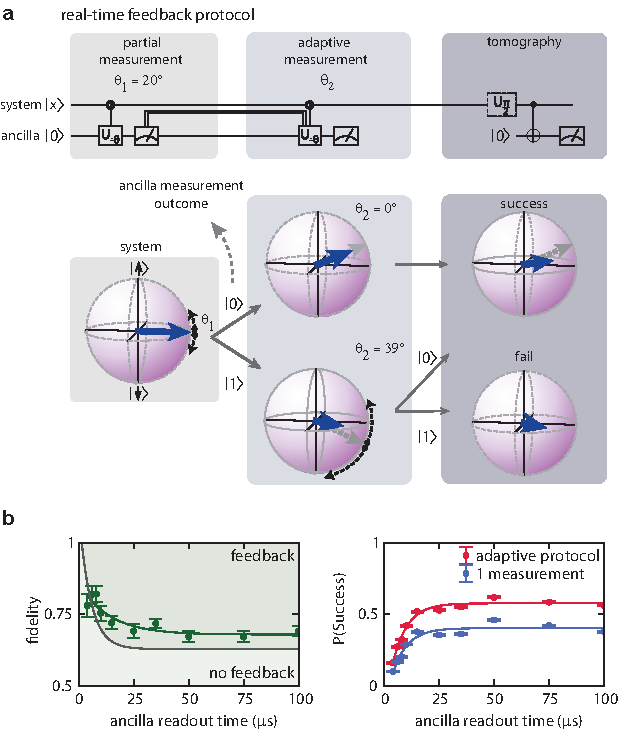
\includegraphics{fig6_adaptive_protocol}
	\caption{\label{fig:amc-fig6} \textbf{Manipulation of a nuclear spin state by sequential partial adaptive measurements with real-time feedback.} (a) Adaptive measurement protocol. The ancilla qubit is initialized in $\ket{0}$ and the system qubit is prepared in $\ket{x}$. The strength of the second measurement ($\theta_2$) is adjusted according to the outcome of the first measurement. The system is analysed by state tomography at each intermediate step. The result of the tomography is plotted on the bloch spheres (blue vector) and compared with the ideal case (grey vector). (b) Fidelity of the output state with respect to the target state as a function of ancilla readout time (dynamical-stop readout) with feedback (only the cases where the protocol heralds success). The grey line is obtained by performing one measurement and adding negative results to artificially increase the success probability to that of the adaptive protocol (red line in right panel). In the right panel we show the probability that the protocol heralds success for one measurement and for the adaptive protocol.  }
\end{figure*}

Our work is the first experimental exploration of a fundamental concept of control-free control \cite{Jordan_PRB_2006, Ashhab_PhysRevA_2010, Wiseman_NatureNV_2011} . Furthermore, the use of adaptive measurements as presented here can increase the performance of spin-based magnetometers \cite{Cappellaro_PhysRevA_2012, Higgins_Nature_2007}. Finally, our results can be combined with recently demonstrated methods for generating entanglement between separate nitrogen vacancy centre spins \cite{Bernien_Nature_2013, Dolde_NatPhys_2013}. Taken together, these techniques form the core capability required for one-way quantum computing, where quantum algorithms are executed by sequential adaptive measurements on a large entangled 'cluster' state \cite{Raussendorf_PRL_2001, Prevedel_Nature_2007}.

%In conclusion, we implemented sequential partial measurements and showed that by adjusting the measurement strength in real-time we can steer a quantum system towards a desired state. Our work is the first experimental exploration of a fundamental concept in the field of quantum measurement and control~\cite{Wiseman_NatureNV_2011} that may find application in systems where control fields are difficult to generate. Furthermore, the use of adaptive measurements as presented here can increase the performance of spin-based magnetometers~\cite{Cappellaro_PhysRevA_2012,Higgins_Nature_2007}. Finally, our results can be combined with recently demonstrated methods for generating entanglement between separate NV center spins~\cite{Bernien_Nature_2013,Dolde_NatPhys_2013}. Taken together, these techniques form the core capability required for one-way quantum computing, where quantum algorithms are executed by sequential adaptive measurements on a large entangled ‘cluster’ state~\cite{Raussendorf_PRL_2001,Prevedel_Nature_2007}.
\newpage
\def\bra#1{\left<#1\right|}
\def\ket#1{\left|#1\right>}
\def\dm#1{\left|#1\right> \left<#1\right|}
\section{Methods}
We use a naturally-occurring nitrogen-vacancy center in high-purity type IIa CVD diamond, with a \textless 111\textgreater-crystal orientation obtained by cleaving and polishing a \textless100\textgreater -substrate. Experiments are performed in a bath cryostat, at the temperature of 4.2 K, with an applied magnetic field of 17 G. Working at low-temperature, we can perform efficient electron spin initialization (F = 0.983 $\pm$ 0.006) and single-shot readout (the fidelity is 0.853 $\pm$ 0.005 for $m_S = 0$ and 0.986 $\pm$ 0.002 for $m_S = -1$) by spin-resolved optical excitation~\cite{Robledo_Nature_2011}. Initialization of the nuclear spin is done by measurement~\cite{Robledo_Nature_2011}, with fidelity  0.95~$\pm$~0.02. Single-qubit operations can be performed with high accuracy using microwave (for the electron) and radio-frequency (for the nucleus) pulses applied to the gold stripline. Note that the single-qubit operations on the nucleus are only used for state preparation and tomography, but not in the feedback protocol. The dephasing time $T_2^*$ is (7.8~$\pm$~0.2)~ms for the nuclear spin and (1.35~$\pm$~0.03)~$\mu$s for the electron spin. 

\subsection{Levels and Hamiltonian}
The NV center forms a natural two qubit system: the electron spin serves as the ancilla qubit, while the system qubit is implemented on the spin of the NV nitrogen atom. The relevant levels are plotted in Fig. \ref{fig:levels}: the full level scheme can be found in the Supporting Online Material of Pfaff \textit{et al}. \cite{Pfaff_NatPhys_2012}.\\
The electron spin is given by the collective spin of the the six unpaired electrons of the negatively-charged state of the center, which constitute a spin $S=1$ system. The $m_s=0$ state is separated from the $m_s=\pm1$ states by the zero-field splitting ($D = 2.878 \pm 0.001$ GHz). The $m_s=-1$ and $m_s=+1$ states are split by $ 98$ MHz by an external magnetic field ($B = 17.5 G$). The ancilla qubit is defined by the $m_s=0  (\ket{0})$ and $m_s=-1  (\ket{1})$ states. Electron spin rotations are performed by microwave pulses, with a Rabi frequency of $ 7.67$ MHz. The probability to excite the $m_s=+1$ spin state when driving microwaves is negligible. The electron spin coherence time has been measured to be $T_2^* = (1.35 \pm 0.03)$ $\mu$s by a Ramsey experiment.\\
The NV's nitrogen atom ($^{14}N$) carries $I=1$ spin and the system qubit is defined by the $m_I = -1 (\ket{\Uparrow})$ and $m_I=0 (\ket{\Downarrow})$ levels, separated in frequency by $\Omega_N = |Q| + g_N \mu_N B \sim 2 \pi \times 5$ MHz, where $Q$ is the nuclear quadrupole splitting $Q = -2\pi \times 4.98 $ MHz. The hyperfine interaction between the electron and nuclear spin has the form $\mathcal{\hat{H}}_{hf} \sim A_z \hat{I}_z \hat{S}_z$ (neglecting small off$-$diagonal terms), which further splits the nuclear levels by an amount $A_z = -2\pi \times 2.184 \pm 0.002$ MHz when the electron is in the $m_s=-1$ manifold.
Nuclear spin rotations are performed by radio-frequency pulses, with a Rabi frequency of $17$ kHz. The nuclear spin coherence time has been measured by a Ramsey experiment to be $T_2^* = 7.8 \pm 0.3$ ms (Fig. \ref{fig:nuclearSpin}).\\

\begin{figure} [h]
\centering
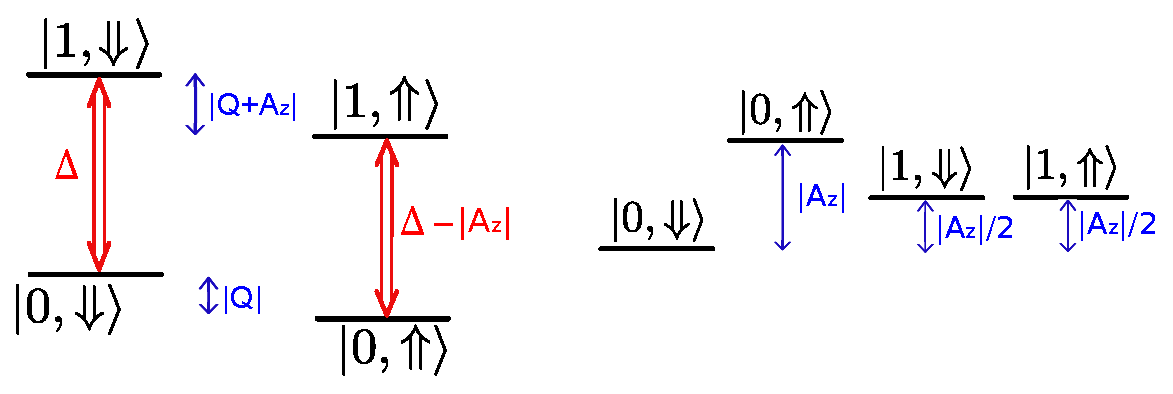
\includegraphics [width = 12 cm]{SOM/fig01_levelScheme.eps}
\caption{\textit{ On the left, scheme of the relevant energy levels for the electron and nuclear spin qubits. On the right, level energies in a doubly-rotating reference frame, rotating at frequency $\omega_e = \Delta-|A_z|/2$ for the electron spin, and $\omega_n = |Q+A_z|$ for the nuclear spin.}}
\label{fig:levels}
\end{figure} 


The Hamiltonian of the system is $\mathcal{\hat{H}}=\mathcal{\hat{H}}_0 +\mathcal{\hat{H}}_{drive}$, with:
\begin{equation}
 \mathcal{\hat{H}}_0 = -|Q| \dm{0, \Uparrow} + \Delta \dm{1, \Downarrow}+(\Delta-|Q+A_z|)\dm{1, \Uparrow}
\end{equation}
and:
\begin{equation}
 \mathcal{\hat{H}}_{drive} = \Omega_{MW} (t)  \hat{S}_{x} \otimes \mathbb{\hat{1}}_N  + \Omega_{RF} (t) \ket{1}\bra{1} \otimes \hat{I}_x + \mbox{h. c.}
 \label{Eq:ham0}
\end{equation}
where $\Delta= D -g_e \mu_eB = 2.8288 \pm 0.0002$  GHz and $\hat{S}_i$, $\hat{I}_i$ are respectively the Pauli operators for the electron spin and the nuclear spin. \\

The Hamiltonian in Eq. \ref{Eq:ham0} is time-dependent and state evolution has, in general, no analytical solution. In order to simplify the problem, we apply the rotating-wave approximation \cite{Slichter__1996}, using a doubly-rotating frame: one rotating at the driving frequency for the electron spin, and the other one at the driving frequency for the nuclear spin. We set the microwave  frequency ($\omega_e = \Delta-|A_z|/2$) such that it is detuned by $|A_z|/2$ from both hyperfine transitions and the RF-field is on resonance with the nuclear spin transition in the $m_s=-1$ electron spin manifold ($\omega_N = |Q+A_z|$). Applying the unitary transformation $\hat{U} = e^{-i \left( \omega_N \mathbb{\hat{1}}_e \times \hat{I}_z + \omega_e \hat{S}_z \times \mathbb{\hat{1}}_N \right) t}$ and retaining the secular terms, the Hamiltonian, in the basis $\{ \ket{0, \Downarrow}, \ket{0, \Uparrow}, \ket{1, \Downarrow}, \ket{1, \Uparrow}  \}$, becomes:

\begin{equation}
\mathcal{\hat{H}'} = \left[
\begin{array}{cccc}
0 & 0 & \Omega^*_{MW} & 0\\
0 & |A_z| & 0 & \Omega^*_{MW}\\
\Omega_{MW} & 0 & |A_z|/2 & \Omega^*_{RF}\\
0 & \Omega_{MW} & \Omega_{RF} & |A_z|/2
\end{array}
\right]
\label{eq:H0_RWA}
\end{equation}

The energy levels, in the rotating-wave approximation, are shown on the right side of Fig. \ref{fig:levels}. We define the positive quantity $A$ to be $A = |A_z|$ in the rest of the Supplementary Information.

\subsection{Qubit initialization}
The electron spin is initialized in the $m_s=0$ state by optical spin-pumping with a fidelity $0.983 \pm 0.006$ \cite{Robledo_Nature_2011}. We use the forbidden transition of $E_{y}$ which is detuned by $\Delta$ from the spin-preserving $E_{y}$-transition. This transition is well suited for a reset of the electron spin during the protocol, since flip-flops with the nuclear spin are suppressed due to selection rules. \\

\begin{figure} [h]
\centering
\includegraphics [width = 12 cm]{SOM/fig02_nuclearSpin_v2.eps}
\caption{\textit{On the left, nuclear spin initialization. The nuclear spin is initially unpolarized (gray): the ESR spectrum for the $m_s=-1 \leftrightarrow 0$ transition shows three hyperfine lines, corresponding to $m_I=-1,0,+1$. By measurement-based initialization (MBI) \cite{Pfaff_NatPhys_2012} we can initialize the spin in any of the nuclear spin states (blue/red). On the right, nuclear spin Ramsey. The nuclear spin is initialized by MBI after which the free evolution time $\tau$ between two $\pi/2$-pulses is varied. The solid line is a fit to the function $y_0 + e^{-(\frac{\tau}{T_{2}^{*}})^2}\cos{(\omega_{det} \tau + \phi )}$ from which we find the dephasing time $T_2^* = 7.8 \pm 0.2$ ms.}}
\label{fig:nuclearSpin}
\end{figure} 

The nuclear spin is initialized by measurement \cite{Pfaff_NatPhys_2012} as shown in Fig. \ref{fig:nuclearSpin}. We prepare the electron spin state in $\left| m_s=\pm 1 \right \rangle$ by spin-pumping on the $E_{y}$ transition. We apply a selective microwave $\pi$-pulse ($f_{rabi} = 181.8$ kHz) to the electron, on resonance with one of the three hyperfine lines. We then read-out the electron spin state, by exciting the $E_y$ transition. In case of photon detection, the electron state is projected to $m_s=0$, and the nuclear spin is projected on the state that was addressed by the microwave pulse.
During the selective microwave pulse, the electron spin undergoes significant dephasing, reducing the success probability, but not the initialization fidelity of the nuclear spin. The measured initialization fidelity is $0.95 \pm 0.02$, obtained from the fitting the heigth of the peaks in Fig. \ref{fig:nuclearSpin}  and the success probability is around $0.07$. The success probability is determined by $p = p_{m_s=-1} \cdot p_{m_I=-1} \cdot p_{e-flip} \cdot p_{phot}$, where the relevant parameters are:
\begin{itemize}
 \item $p_{m_s=-1} \sim 0.5$ is the probability to spin pump the electron spin in $m_s=-1$ (in the remaining cases it's in $m_s = +1$).
 \item $p_{m_I=-1} \sim 1/3$ is the population of the desired state $m_I=-1$ for an initially unpolarized nuclear spin.
 \item $p_{e-flip} \sim 0.6$ is the success probability of nuclear-dependent electron spin rotations.
 \item $ p_{phot} \sim 0.6-0.8$ is the probability to detect a photon when reading-out the $m_s=0$ state, limited by the collection of the optical system and the finite photon detection efficiency.
\end{itemize}


\subsection {Nucleus-independent electron spin rotations}

The maximum Rabi frequency we achieve in the setup is $\sim 8$ MHz (Fig. \ref{fig:rabi}). Given the hyperfine splitting of 2.184 MHz, these pulses introduce off-resonant driving errors that limit the weakest measurement we could achieve to $\theta = 15$ degrees ($C = 0.27$, see equation \ref{eq:concurrence}). To overcome this problem, we use CORPSE pulses \cite{Cummins_PRA_2003}, a composite pulse sequence designed to compensate for off-resonance errors. The weakest measurement we achieve with the CORPSE pulses is $\theta_{min} = 5$ degrees, corresponding to $\tau = 12$ ns (obtained from a fit of the Ramsey fringes in Fig. \ref{fig:amc-fig1}b of the main text)

\begin{figure} 
\centering
\includegraphics [width = 12 cm]{SOM/rabi.eps}
\caption{\textit{Coherent single-qubit rotations of the electron spin ancilla qubit (orange) and the nuclear spin system qubit (purple) are performed by varying the length of a MW (RF) pulse. Solid lines are sinusoidal fits from which we determine the Rabi frequency  $7.67 \pm 0.02$ MHz / $17.07 \pm 0.01$ kHz).}}
\label{fig:rabi}
\end{figure} 

\subsection{Electron-independent nuclear spin rotation}
\label {sec:uncond_rot_RF}
For quantum state tomography and for weak-value measurements, we need to be able to perform nuclear spin rotations, unconditional on the electron spin state. This is not trivial if the electron and nuclear spins are entangled.
In particular, when the electron is in the $\left| m_s=-1 \right \rangle$ state, the splitting between $\left| \Downarrow \right \rangle$ and $\left| \Uparrow \right \rangle$ is $\omega_N^{(-1)} = |Q+A_z| = 2\pi \times 7.164$ MHz, while when the electron in the $\left| m_s=0 \right \rangle$ state, $\omega_N^{(0)} = |Q| = 2\pi \times 4.98$ MHz. Given that the Rabi frequency of the nuclear spin is much smaller than the hyperfine interaction, the simple use of a hard $\pi$-pulse, as done for the electron, does not work. \\
We implemented the unconditional nuclear spin rotation using the scheme depicted in Fig. \ref{fig:RF}a. First we apply an RF pulse (RF-1) at $\omega_N^{(-1)}$, to rotate the nuclear spin when the electron spin is in the $\left| m_s=-1 \right \rangle$ manifold. We then apply a hard $\pi$-pulse to the electron and apply a second RF pulse (RF-2) at the same frequency $\omega_N^{(-1)}$.\\
As explained in Section \ref{sec:theory} (Eq. \ref{eq:state}), the partial measurement introduces a phase shift to the system qubit that depends on the measurement strength. The phase shift is proportional to the interaction time $\tau$ of the measurement. In order to characterize the phase shift, we used the following protocol:
\begin{itemize}
 \item we set the pulse length of RF-1 and RF-2 corresponding to a $\pi/2$ pulse ($T_{RF-1/2} = 14.6 \mu$s)
 \item we only apply the RF-1 pulse and sweep the phase of RF-1 for different values of $\tau$. Fitting the resulting sinusoidal signal, we recover the phase offset $\varphi_0^{(RF-1)} (\tau)$
 \item we then set the amplitude of RF-2 to the value corresponding to a $\pi/2$-pulse and without RF-1 apply a $\pi$-pulse on the electron followed by RF-2. We then sweep the phase of RF-2 for different values of $\tau$ and fit the sinusoid to reconstruct the phase offset $\varphi_0^{(RF-2)} (\tau)$
\end{itemize}
The values of the phase offsets as a function of $\tau$ for RF-1 and RF-2 ($\varphi_0^{(RF-1)} (\tau)$ and $\varphi_0^{(RF-1)} (\tau)$) are plotted in Fig. \ref{fig:RF}b. These values can be used to make sure that the resulting entangled nuclear-electron state has the correct phase when performing quantum state tomography (projections along $x$ and $y$ with a $\pi/2$-pulse along the corresponding axis and projection along $z$).\\
Furthermore, care should be taken that in general, while applying the first RF pulse (which rotates the nuclear spin by an angle $\Phi$ conditioned on the electron being in $\left| m_s=-1 \right \rangle$), the nuclear spin in the electron $ m_s=0$ manifold will undergo free-evolution, acquiring an additional phase shift proportional to the temporal length of the pulse (therefore to $\Phi$). Therefore, we need to characterize this phase offset for all situations different from a $\pi/2$-pulse. This was done by fixing $\tau$ and sweeping the phase of RF-2 for different value of the length of the RF-1 pulse ($T_{RF-1}$). After fitting the resulting sinusoidal oscillation, we retrieved the extra phase offset $\varphi_2 (\Phi)$ to RF-2 such that it is applied in the correct rotating frame. 

\begin{figure} [h]
\includegraphics [width = 12 cm]{SOM/fig03_RFpulses_v2.eps}
\caption{\textit {On the left, pulse sequence for unconditional nuclear spin rotation. On the right, phase of the nuclear spin as a function of the free evolution time $\tau$, for the two electron-spin manifolds ($m_S=-1$ and $m_S=0$).}}
\label{fig:RF}
\end{figure} 



\subsection{Partial measurements with controlled strength: Theory}
\label{sec:theory}
The protocol starts by initializing the nucleus in $\ket{\psi_N} = \frac{1}{\sqrt{2}} \left( \ket{\Downarrow}+\ket{\Uparrow} \right)$ and the electron in $\ket{\psi_e} = \ket{0}$.\\
The tunable-entangling gate consists of three steps. First, a $\pi/2$-pulse is applied around $x$ to the electron spin, creating the equal superposition state:
\begin{equation}
\left| \psi \right \rangle = \frac{1}{2} \left( \left| 0 \right \rangle - i \left| 1 \right \rangle \right) \left( \left| \Downarrow \right \rangle +\left| \Uparrow \right \rangle\right)
\end{equation}
Then the system undergoes free evolution of a variable time $\tau$ (according to the Hamiltonian in Eq. \ref{eq:H0_RWA}):
\begin{equation}
\ket{ \psi} = \frac{1}{2} \left \lbrace e^{0i} \ket{ 0, \Downarrow } + e^{-i A \tau} \ket{ 0, \Uparrow } - i  e^{-i A \tau/2} \ket{ 1, \Downarrow } - i  e^{-i A \tau/2} \ket{ 1, \Uparrow} \right \rbrace
\end{equation}
A second electron $\pi/2$-pulse, now around $y$, creates the state:
\begin{equation}
\left| \psi \right \rangle = \frac{1}{2} \left\lbrace \left| 0 \right \rangle \left[ \beta_+ (\tau) \left| \Downarrow \right \rangle + i e^{i A\tau/4} \beta_-(\tau) \left| \Uparrow \right \rangle \right] + e^{i\pi /2} \left| 1 \right \rangle \left[ \beta_-(\tau) \left| \Downarrow \right \rangle + i e^{i A\tau/4} \beta_+(\tau) \left| \Uparrow \right \rangle \right] \right\rbrace
\label{eq:state}
\end{equation}
where $\beta_{\pm} = \cos(\pi/4 \pm  A \tau/4)$. We define $\theta$ as $\theta= A \tau/2$, and the measurement strength as $\sin\theta$.\\
For $\theta=0$ ($\tau = 0$), the electron and nuclear spins are in a separable state:
\begin{equation}
\left| \psi (\tau=0) \right \rangle = \frac{1}{2} \left( \left| 0 \right \rangle +i \left| 1 \right \rangle \right) \left[ \left| \Downarrow \right \rangle +  i \left| \Uparrow \right \rangle \right]
\end{equation}
and a measurement of the electron spin gives no information about the state of the nuclear spin.
On the other hand, for $\theta = 90$ degrees (corresponding to $\tau = \pi/A = 229$ ns), the electron and nuclear spins are in a maximally-entangled state:
\begin{equation}
\left| \psi (\tau=\pi/A) \right \rangle = \frac{1}{\sqrt{2}} \left[ \left| 0, \Uparrow \right \rangle -i \left| 1, \Downarrow \right \rangle \right]
\end{equation}
and a measurement of the electron spin results in a projective measurement of the nuclear spin. Performing the electron-spin read-out by resonantly exciting the $E_y$ optical transition (therefore probing the population of the $\left| m_s=0 \right \rangle$ state) we project the nuclear spin on the $\left| m_I = -1 \right \rangle$ ($\ket{\Uparrow}$) state when a photon is detected and on the $\left| m_I = 0 \right \rangle$ ($\ket{\Downarrow}$) state when no photon is detected.\\
In the intermediate cases, $0<\tau<\pi/A$, the concurrence of the state as a function of $\tau$ is given by:
\begin{equation}
 C (\tau) = \sin\theta=\sin \left( A \tau/2 \right) 
\label{eq:concurrence}
\end{equation}
if $\ket{\psi_N}$ is initialized in $\ket{x}$. The value of C corresponds to the strength of the measurement performed on the system qubit.\\
Note from Eq. \ref{eq:state} that a $\tau$-dependent phase shift $\varphi = + A \tau/4$, unconditional on the electron spin, is imposed on the nuclear spin state after the measurement, as a result of the variable free evolution time. We compensate by adjusting the phase of the final RF pulse (see Section \ref{sec:uncond_rot_RF} for details).\\
The nuclear spin density matrix, unconditioned on the result of the electron spin measurement, can be derived by tracing over the electron spin, resulting in:
\begin{equation}
 \rho_{uncond} = \frac{1}{2}
 \left[
% \begin{center}
\begin{array}{cc}
1 & \cos^2 ( A \tau/2)\\
\cos^2 ( A \tau/2) & 1
 \end{array}
% \end{center}
 \right]
\label{eq:uncondRho}
 \end{equation}
Increasing the measurement strength, the initial pure state becomes increasingly mixed, resulting in a completely mixed state for $\theta = 90$ degrees.\\
 Conditioning on measuring the electron spin in the state $\ket{0}$, the nuclear spin state is:
\begin{equation}
 \rho_0 = \frac{1}{2}
 \left[
% \begin{center}
\begin{array}{cc}
1+\sin ( A \tau/2) & \cos^2 ( A \tau/2)\\
\cos^2 ( A \tau/2) & 1-\sin(A \tau/2)
 \end{array}
% \end{center}
 \right]
 \label{eq:condRho}
\end{equation}
Now, the resulting state remains pure, but it is increasingly rotated towards $\ket{\Uparrow}$ for increasing measurement strength. 

\subsection{Characterization of the partial measurements}
The partial measurement was characterized by performing quantum state tomography, as explained in the main text. In Fig \ref{fig:backaction}, we plot the elements of the density matrix of the nuclear spin after the partial measurement as a function of the measurement strength, for three different input states $\{ \ket{\Uparrow}, \ket{x}, \ket{y} \}$. On the upper row we do not take the measurement outcome of the electron into account, while on the lower row we show the data conditioned on the detection of a photon (ancilla projected to $\ket{0}$).\\
When we condition on a measurement result for the ancilla, the operation on the system qubit is a projection with increasing strength (completely projective along $z$ for measurement strength 1). In the unconditioned case, we observe measurement-induced dephasing.

\begin{figure} 
\includegraphics [width = 12 cm]{SOM/fig04_backAction.eps}
\caption{\textit{Density matrix elements of the states after a partial measurement, as a function of the measurement strength, for three different input states. On the upper row, data not taking the electron spin readout into account. On the lower row, data conditioned on detection of a photon (electron spin projected to $m_s = 0$). Solid lines represent theoretical prediction from Eq. \ref{eq:uncondRho} and Eq. \ref{eq:condRho}}}
\label{fig:backaction}
\end{figure} 


We characterized the collapse process by quantum process tomography \cite{Nielsen__2000}. Results are plotted in Fig. \ref{fig:QPT}. On the upper row, the process matrix for the unconditioned case shows a continuous transition from the identity process to a collapse process consisting of equal contributions of $\mathbb{\hat{1}}$ and $\hat{\sigma}_z$: the absence of off-diagonal terms represents the increasing dephasing. The theoretical process matrix for the unconditioned case is:
\begin{equation}
 \hat{\chi}_{uncond} = \frac{1}{2}
 \left[
\begin{array}{cccc}
1+\cos\theta & 0 & 0 & 0\\
0 & 0 & 0 & 0\\
0 & 0 & 0 & 0\\
0 & 0 & 0 & 1-\cos\theta
 \end{array}
 \right]
\end{equation}
On the bottom row, we plot the process conditioned on the measurement result of the electron spin: this is a non-trace-preserving process, with state-dependent success probability \cite{Bongioanni_Phys.Rev.A_2010}. The theoretical process matrix as a function of $\theta$ is:
\begin{equation}
\hat{\chi}_{cond} = \frac{1}{2}
 \left[
\begin{array}{cccc}
1+\cos\theta & 0 & 0 & \sin\theta\\
0 & 0 & 0 & 0\\
0 & 0 & 0 & 0\\
\sin\theta & 0 & 0 & 1-\cos\theta
 \end{array}
 \right]
\end{equation}
In this case, the process is coherent and the off-diagonal terms are, in general, non-zero. The fidelity between the ideal process matrix and our experimentally reconstructed one is plotted in Fig. \ref{fig:QPT_fid}.


\begin{figure} 
\centering
\includegraphics [width = 12 cm]{SOM/fig05_QPT.eps}
\caption{\textit{ Quantum process tomography for the tunable-strength measurement for different strength values (defined by the value of $\tau$ and the corresponding values for $\theta =  A \tau/2$ and measurement strength $C=\sin\theta$). On the upper row, the real part of the process matrix for the unconditioned case. On the lower row, the process matrix conditioned on a measurement of the ancilla giving the result $\ket{0}$.}}
\label{fig:QPT}
\end{figure} 


\begin{figure} 
\centering
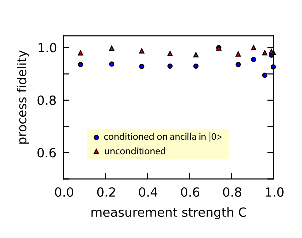
\includegraphics [width = 6 cm]{SOM/fig06_QPTfidelity.eps}
\caption{\textit{ Fidelity of the reconstructed quantum process matrices $\chi_{cond}$ and $\chi_{uncond}$, as a function of the measurement strength ($C = \sin\theta$). The fidelity is calculated with the formula: $F (\chi_{exp}, \chi_{th})  = \mbox{Tr} \left \lbrace \sqrt{\sqrt{\chi_{exp}} \chi_{th} \sqrt{\chi_{exp}}} \right\rbrace^2$ \cite{Bongioanni_Phys.Rev.A_2010}.}}
\label{fig:QPT_fid}
\end{figure} 

\subsection {Weak value and conditioned average}
Given an observable $\mathcal{I}$, the weak value of the associated quantum operator $\hat{I}$, as introduced by Aharonov, Albert and Vaidman \cite{Aharonov_PRL_1988,Kofman_PhysicsReports_2012}, is defined by

\begin{equation}
\label{eq:wv}
 I_W = \frac{ \bra{\psi_f} \hat{I} \ket{\psi_i}}{\left \langle \psi_f | \psi_i \right \rangle }
\end{equation}
This quantity does not depend on the context of the specific measurement, but only on the operator $\hat{A}$ and on the initial and final states (respectively $\left| \psi_i \right \rangle$ and $\left| \psi_f \right \rangle$). For a qubit, with initial state $\ket{\psi_i} = \ket{x}$ and final state $\ket{\psi_f}  = \cos \phi \ket{0} + \sin \phi \ket{1}$, we have $(S_z)_w = \cos 2\phi/(1+\sin 2\phi)$.\\
Given an observable $\mathcal{A}$, one can measure it with a series of operators, which can be projectors $\lbrace \hat{\Pi}_k , \hat{\Pi}_k^2 = \hat{\Pi}_k\rbrace$ or, more generally, POVMs $\lbrace \hat{E}_j = \hat{M}^{\dagger}_j \hat{M}_j \rbrace$. The associated measurement outcomes are, respectively, the eigenvalues $\left \lbrace a_k \right \rbrace$ and the generalized eigenvalues (or contextual values) $\left \lbrace \alpha_j \right \rbrace$ \cite{Dressel_Phys.Rev.Lett._2010}, such that the spectral decomposition of the operator $\hat{I}$ can be written as:
\begin{equation}
 \hat{I} = \sum_j \alpha_j \hat{E}_j = \sum_k a_k \hat{\Pi}_k
\end{equation}


Consider now a sequence of two measurements, $\mathcal{M}_1$ and $\mathcal{M}_2$ and suppose to condition the average of the result of  $\mathcal{M}_1$ to a measurement result for $\mathcal{M}_2$. The generalized weak value (or conditioned average) of the observable is defined as:
\begin{equation}
 _f \left \langle I \right \rangle = \sum_j \alpha_j^{(1)} P(j|f)
\end{equation}
where $\lbrace \alpha_j^{(1)}\rbrace$ are the possible measurement outcomes of $\mathcal{M}_1$ (generalized eigenvalues) and $P(j|f) = p_{jf}/(\sum_j p_{jf})$ is the conditional probability to detect the outcome $\alpha_j^{(1)}$ in the first measurement, given the outcome $\alpha_f^{(2)}$ for the second measurement.\\
Unlike the weak value, the conditioned average encodes information not only about the observable $\mathcal{A}$, but also on the specific measurement context. However, it can be shown \cite{Dressel_Phys.Rev.Lett._2010} that, under certain conditions (namely minimal state disturbance), the dependence on the measurement vanishes. For a pure initial state, a pure POVM and a projective final measurement, it reduces to the weak value of Eq. \ref{eq:wv} .\\
In our case, for a measurement operator $\hat{E}_j = (1/2) (\mathbb{\hat{1}} \pm \sin\theta \hat{I}_z)$, the generalized eigenvalues are $\pm 1/\sin\theta$ and the conditional average is:
\begin{equation}
\label{eq:cond_avg}
 _f \left \langle I_z \right \rangle = \frac{1}{\sin\theta} \frac{p_{00}-p_{10}}{p_{00}+p_{10}}  = \frac{\cos 2\phi}{1+ \cos \theta \sin 2\phi}
\end{equation}
This quantity reduces to the quantum weak value for $\sin\theta = 0$ and does not diverge for finite measurement strength. Note that from this expression \cite{Williams_PRL_2008,Groen_PRL_2013}, it is possible to observe values lying outside the range of the operator eigenvalues for any finite measurement strength.
\\

\subsection {Experimental quantum weak value for a spin qubit}
A measurement of the conditional average $ _f \left \langle I_z \right \rangle$ is performed with the pulse sequence shown in Fig. \ref{fig:amc-fig1}a of the main text, starting from the initial state $\ket{x} = (1/\sqrt{2}) \left( \ket{\Downarrow} + \ket{\Uparrow} \right)$. The scheme consists of a partial measurement (strength $\theta$) followed by a projective measurement in a rotated basis (angle $\phi$), post-selecting on the result of the projective measurement. In the first set of measurements (large panel in Fig. \ref{fig:amc-fig2}d of the main text) we fix the strength of the first measurement and sweep the basis rotation angle $\phi$ before the projective measurement. For the inset of Fig. \ref{fig:amc-fig2}d of the main text we sweep the measurement strength $\theta$ and choose $\phi$ to yield the maximum weak value. \\
We post-select on the measurement outcome $\ket{0}$ for the ancilla read-out (system in $\ket{\Uparrow}$), corresponding to the detection of a photon (electron spin in $m_s=0$). \\
The conditional average can be calculated with the expression in Eq. \ref {eq:cond_avg} where $p_{ij}$ is the probability of outcome $i$ for the ancilla read-out of the partial measurement and measurement outcome $j$ for the ancilla read-out of the projective measurement (assuming perfect readout). From Eq. \ref{eq:state}, we calculate the dependence of $p_{ij}$ on $\phi$ and $\theta$:
\begin{equation}
\label{eq:prob_wm}
  \begin{split}
  p_{11}&=\frac{1}{2} \left[ \beta_-(\theta) \cos\phi + \beta_+ (\theta) \sin\phi \right]^2  \\
  p_{10}&= \frac{1}{2} \left[ \beta_-(\theta) \sin\phi - \beta_+ (\theta) \cos\phi\right]^2 \\
  p_{01}&= \frac{1}{2} \left[ \beta_-(\theta) \sin\phi + \beta_+ (\theta) \cos\phi\right]^2 \\
  p_{00}&=\frac{1}{2} \left[ \beta_-(\theta) \cos\phi - \beta_+ (\theta) \sin\phi \right]^2 
  \end{split}
\end{equation}
where $\beta_{\pm} (\theta) = \cos (\pi/4 \pm \theta/2)$.\\
 
Since our read-out is not perfect, it must be calibrated to take into account the finite detection efficiency and the dark counts. For the state $m_s=0$ we are limited by our detection efficiency ($\sim .80$), while for the $m_s=-1$ read-out we suffer from dark counts. We define $F_i$ as the fidelity of the $m_s=0$ read-out and $G_i$ as the read-out fidelity for $m_s=-1$, in the $i-$th measurement.
Then, given the ideal probabilities $p_{ij}$, the measured fractions $n_{ij}$ are:
 
\begin{equation}
\resizebox{.9\hsize}{!}{$
\left[
\begin{array}{c}
n_{11}\\
n_{10}\\
n_{01}\\
n_{00}
 \end{array}
 \right]=
 \left[
\begin{array}{cccc}
G_1 G_2 & G_1(1-F_2) & (1-F_1)G_2 & (1-F_1)(1-F_2)\\
G_1(1-G_2) & G_1 F_2 & (1-F_1)(1-G_2) & F_2(1-F_1)\\
(1-G_1)G_2 & (1-G_1)(1-F_2) & F_1 G_2 & F_1(1-F_2)\\
(1-G_1)(1-G_2) & (1-G_1)F_2 & F_1 (1-G_2) & F_1 F_2
 \end{array}
 \right]
\left[
\begin{array}{c}
p_{11}\\
p_{10}\\
p_{01}\\
p_{00}
 \end{array}
 \right] $}
\label{ROcor}
\end{equation}
The theoretical curve in Fig. \ref{fig:amc-fig2}d of the main text is calculated without fit-parameters, using the read-out correction of Eq. \ref{ROcor} and assuming an asymmetric spin-flip rate $f= 0.02$ between the first and second read-out. This spin-flip probability arises during the reset of the ancilla by optically exciting the forbidden transition of Ey. The value $f$ is determined from independent measurements. \\


\subsection{Partial measurements as probabilistic rotations}
Starting from the state $\ket{\psi_{init}} =  \cos\theta_i \ket{\Downarrow}+ \sin\theta_i \ket{\Uparrow} $, we perform a partial measurement with strength $\theta_m$. With probability $\cos^2\theta$, we obtain the state:
\begin{equation}
 \ket{\psi_0} = \frac{1}{\mathcal{N}_0} \left[ \cos \left( \pi/4 + \theta_m/2 \right) \cos\theta_i \ket{\Downarrow} +  \cos \left( \pi/4 - \theta_m/2 \right) \sin\theta_i \ket{\Uparrow} \right]
\end{equation}
where $1/\mathcal{N}_0$ is the normalization factor. The state, initially at an angle $\theta_i$, is rotated to the angle:
\begin{equation}
 \theta_0 = \arctan{ \left[ \tan\theta_i \frac{\cos\theta_m}{1-\sin\theta_m} \right]}
\end{equation}
On the other hand, with probability $p_{succ} = \sin^2\theta$, the measurmeent leads to the state:
\begin{equation}
 \ket{\psi_1} = \frac{1}{\mathcal{N}_1} \left[ \cos \left( \pi/4 - \theta_m/2 \right) \cos\theta_i \ket{\Downarrow} +  \cos \left( \pi/4 + \theta_m/2 \right) \sin\theta_i \ket{\Uparrow} \right]
\end{equation}
Therefore, the initial state rotated to the angle:
\begin{equation}
 \theta_1 = \arctan{ \left[ \tan\theta_i \frac{1-\sin\theta_m}{\cos\theta_m} \right]}
\end{equation}
In other words, as shown in \cite{Jordan_PRB_2006}, a partial measurement is equivalent to a probabilistic state rotation, with a rotation angle which depends on the strength of the measurement and on the initial state (see Fig. \ref{fig:prob_rot}).

\begin{figure} 
\centering
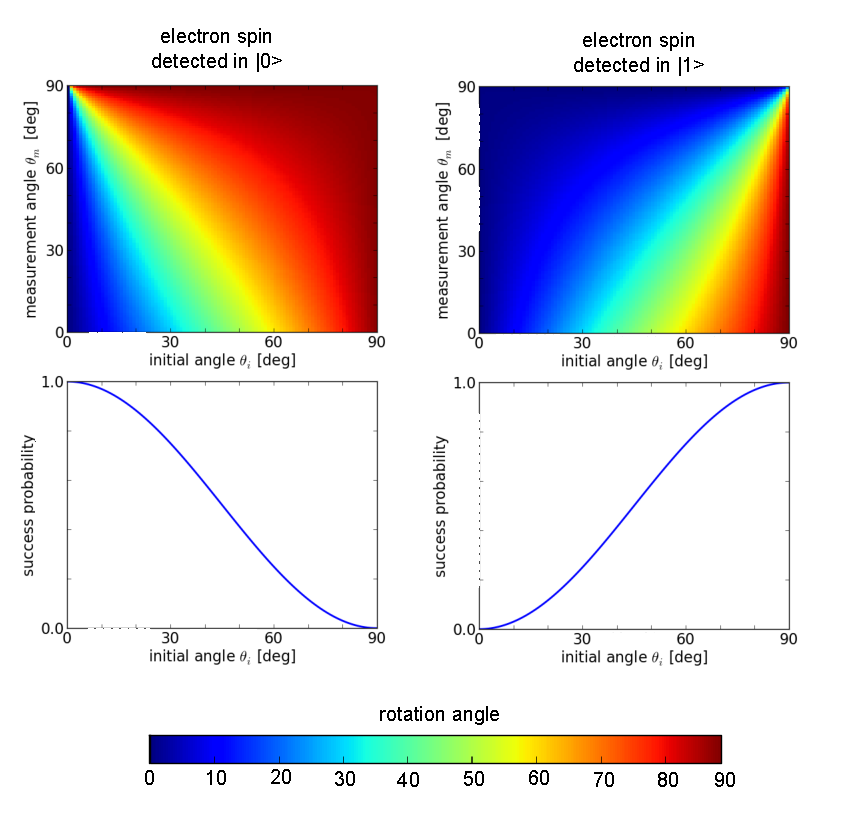
\includegraphics [width = 12 cm]{SOM/fig07_prob_rotation.eps}
\caption{\textit{A partial measurement is equivalent to a probabilistic rotation. Given a an initial superposition with angle $\theta_i$ ($\ket{\psi_{init}} =  \cos\theta_i \ket{\Downarrow}+ \sin\theta_i \ket{\Uparrow} $) and a partial measurement with strength $\theta_m$, one gets the rotation angle plotted on the upper left subplot in case the electron spin is measured to be in $\ket{0}$ (probability $\cos^2 \theta_i$, plot on the bottom left) or the rotation angle plotted on the upper right in case the electron spin is measured to be in $\ket{1}$ (probability $\sin^2 \theta_i$, plot on the bottom right)}}
\label{fig:prob_rot}
\end{figure} 


\subsection{Heralded sequential measurements: un-collapse and steering}
In Fig. \ref{fig:uncollapse}, we implement two heralded sequential partial measurements. We post-select on the case of photon detection, using short read-out times to minimize electron spin-flips, at the price of reduced success probabilities. We can do this with high fidelity, maintaining a good coherence of the state after two measurements. No spin-pumping between the two measurements is performed, in order to avoid electron spin-flips that would destroy nuclear-spin coherence.\\
We first perform a measurement with strength $\theta_1=20$ degrees, followed by a measurement with the same strength but projecting on the opposite electron state (equivalent to a measurement with strength $\theta_2=-20$ degrees). This brings us back to the original quantum state, in a probabilistic un-collapse of the state. This technique has been used to probabilistically recover a state subject to amplitude-damping decoherence \cite{Koashi_Phys.Rev.Lett._1999,Korotkov_Phys.Rev.Lett._2006,Katz_Phys.Rev.Lett._2008}.  \\
In general, a partial quantum measurement is equivalent to a probabilistic rotation. For $\theta_1=\theta_2=+20$ degrees, two successive measurements result in a combined rotation of $39$ degrees, with success probability $0.16$. In our case, heralding on photon detection, this can be done quite effectively (fidelity $0.78$).

\begin{figure} 
\centering
\includegraphics [width = 12 cm]{SOM/fig08_uncollapse.eps}
\caption{\textit{Two sequential heralded partial measurements, both post-selected on the case of photon detection. The density matrices are the result of state tomography, performed after the two partial measurements. For the uncollapse (upper density matrix), first a measurement with strength $C = 0.34$ ($\theta_1=20$ degrees) is performed, after which the initial state is restored by a second measurement with $\theta_2 = -20$ degrees. For the lower density matrix, the second measurement is set to  $\theta_2 = 39$ degrees, such that the system, that was projected towards $|\downarrow >$ after the first measurements,  is steered towards $|\uparrow >$ through the backaction of the second measurement.}}
\label{fig:uncollapse}
\end{figure} 

\section{State steering by real-time adaptive measurements}
\subsection{Ideal protocol}
We start in the state $\left| \psi_0 \right \rangle = \ket{x} = (1/\sqrt{2}) \left(\left| \Downarrow \right \rangle + \left| \Uparrow \right \rangle \right)$, with the goal to reach a target state $\left| \psi_T \right \rangle = \cos\theta_T \left| \Downarrow \right \rangle + \sin\theta_T \left| \Uparrow \right \rangle$.\\
First, we do a measurement with strength $\theta_1 = \pi/2-2\theta_T$. With probability $0.5$ the system reaches the target state, while in the rest of the cases it is shifted in the oppposite direction, to the state:
\begin{equation}
\left| \psi_1 \right \rangle = \cos \left( \frac{\pi}{4} - \frac{\theta_1}{2} \right) \left| \Downarrow \right \rangle + \cos \left( \frac{\pi}{4} + \frac{\theta_1}{2} \right) \left| \Uparrow \right \rangle
\end{equation}
In order to try to steer it back, we perform a second measurement, with strength $\theta_2$. In case of success, we get the state:
\begin{equation}
\resizebox{.9\hsize}{!}{$
\left| \psi_{10} \right \rangle = \frac{1}{\mathcal{N}} \left[ \cos \left( \frac{\pi}{4} - \frac{\theta_1}{2} \right)\cos \left( \frac{\pi}{4} + \frac{\theta_2}{2} \right) \left| \Downarrow \right \rangle + \cos \left( \frac{\pi}{4} + \frac{\theta_1}{2} \right)\cos \left( \frac{\pi}{4} - \frac{\theta_2}{2} \right) \left| \Uparrow \right \rangle \right]
$}
\end{equation}
where $\mathcal{N} = \left[ \cos^{2} \left( \frac{\pi}{4} - \frac{\theta_1}{2} \right)\cos^2 \left( \frac{\pi}{4} + \frac{\theta_2}{2} \right) + \cos^2 \left( \frac{\pi}{4} + \frac{\theta_1}{2} \right) \cos^2 \left( \frac{\pi}{4} - \frac{\theta_2}{2} \right) \right]^{1/2}$.
The system can be steered to target state, by setting:
\begin{equation}
 \frac{1}{\mathcal{N}} \cos \left( \frac{\pi}{4} - \frac{\theta_1}{2} \right)\cos \left( \frac{\pi}{4} + \frac{\theta_2}{2} \right) = \cos \left( \frac{\pi}{4} + \frac{\theta_1}{2} \right)
\end{equation}
After simplification, this leads to the equation:
\begin{equation}
\left( 1 + \sin \theta_1 \right) \left( 1 - \sin \theta_2 \right) = \left( 1 - \sin \theta_1 \right) \left( 1 - \sin \theta_1 \sin \theta_2 \right)
\end{equation}
Solving for $\theta_2$, we find that the strength of the second measurement can be tuned as:
\begin{equation}
 \theta_2 =  \sin^{-1} \left[ 2\frac{\sin \theta_1}{1+\sin^2 \theta_1} \right]
\end{equation}
The probability to steer the state to the desired target, after two measurements, is:
\begin{equation}
 p_{success} = \frac{ 1 + \cos \theta_1 }{2}
\end{equation}


\begin{figure} 
\centering
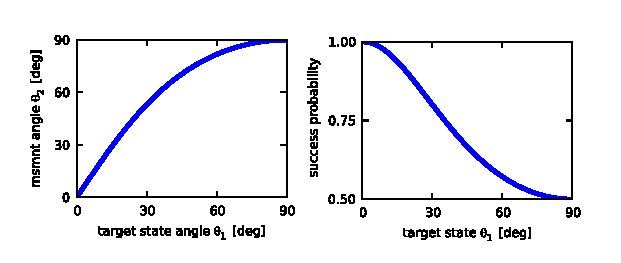
\includegraphics [width = 12 cm]{SOM/fig09_adaptMsmsnt_angle.eps}
\caption{\textit{On the left, strength of the second measurement, as a function of the desired target state. On the right, success probability of the two-step algorithm.}}
\label{}
\end{figure} 


\subsection{Error analysis}
The protocol described in the last Section assumes ideal measurements. In practice, however, we are subject to several non-ideal conditions \cite{Robledo_Nature_2011}:
\begin{itemize}
 \item the electron-spin read-out is not perfect. Given that the electron is in $m_s=0$, if we excite the $E_{y}$ transition, we are supposed to detect photons. However, such photons are detected with a finite efficiency (due to losses in the diamond, the collection optics and the finite efficiency of the detector). This results in a read-out fidelity $F_0 < 1$. In the first measurement, this leads us to make the wrong decision and apply a correction although we had already reached the target state.
 \item due to dark counts, we detect photon clicks even in the absence of photons. This probability is quite small, so we neglect it in the following analysis
 \item during electron read-out, there is a probability ($q$) that the electron spin flips. This results in dephasing of the nuclear spin. Moreover, with a small probability it results also in a nuclear spin-flip (we measured the probability to get a nuclear spin-flip as a result of an electron spin-flip to be around $0.02$). We neglect the nuclear spin flip and just consider the effect of dephasing.
\end{itemize}

The read-out efficiency and spin-flip probability are not independent: the longer the read-out, the higher the detection efficiency, but, at the same time, the electron spin-flip probability is also increased. The read-out fidelity $F_0$ and the electron spin-flip probability $q$, as a function of read-out time, are shown in the inset of Fig. \ref{fig:adaptiveScheme}. The best trade-off is for a read-out time $T \sim 5 \mu$s, where $F_0 \sim 0.6$ and $q \sim 0.2$.

\begin{figure} 
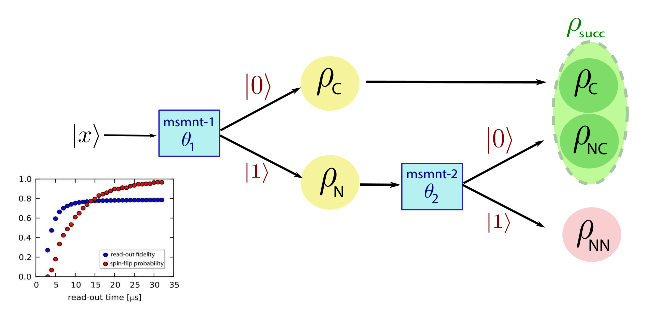
\includegraphics [width = 12 cm]{SOM/fig10_adaptiveScheme.eps}
\caption{\textit{Description of the adaptive scheme. Ancilla readout $\ket{0}$ corresponds to the detection of a photon when optically exciting the $E_{y}$ transition, while no photon detection corresponds to ancilla projection to $\ket{1}$. Inset: experimental data for electron spin read-out fidelity $F_0$ and spin-flip probability $q$ as a function of read-out time.}}
\label{fig:adaptiveScheme}
\end{figure} 

\newpage
\bibliographystyle{../thesis}
\bibliography{amc}


